\documentclass{article}
\usepackage[margin=1in]{geometry}
\usepackage{amsmath,amsthm,amssymb}
\usepackage{bbm,enumerate,mathtools}
\usepackage{tikz,pgfplots}
\usepackage{chessboard}
\usepackage[hidelinks]{hyperref}
\usepackage{multicol} % Problem 35

\newenvironment{question}{\begin{trivlist}\item[\textbf{Question.}]}{\end{trivlist}}
\newenvironment{note}{\begin{trivlist}\item[\textbf{Note.}]}{\end{trivlist}}
\newenvironment{references}{\begin{trivlist}\item[\textbf{References.}]}{\end{trivlist}}
\newenvironment{related}{\begin{trivlist}\item[\textbf{Related.}]\end{trivlist}\begin{enumerate}}{\end{enumerate}}


\begin{document}
\rating{2}{1}
Consider an $n \times n$ chess board, with pieces that can move integer
distances, but only in diagonal directions---that is, they move like the
hypotenuse of a Pythagorean triangle.
\begin{figure}[!h]
  \centering
  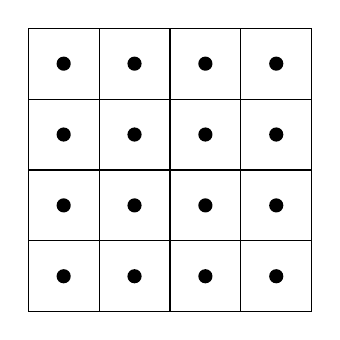
\begin{tikzpicture}[scale=0.9]
    \draw (0,0) grid (4,4);
    \foreach \x in {0,1,2,3} {
      \foreach \y in {0,1,2,3} {
        \fill (\x + 0.5, \y + 0.5) circle (0.1 cm);
      }
    }
  \end{tikzpicture} \hspace{1cm}
  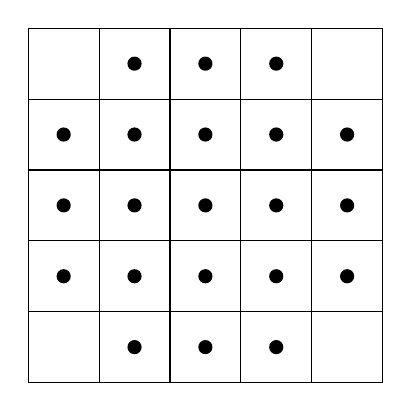
\begin{tikzpicture}[scale=0.9]
    \draw (0,0) grid (5,5);
    \foreach \x in {1,2,3} {
      \foreach \y in {0,1,2,3,4} {
        \fill (\x + 0.5, \y + 0.5) circle (0.1 cm);
      }
    }
    \foreach \y in {1,2,3} {
      \fill (0 + 0.5, \y + 0.5) circle (0.1 cm);
      \fill (4 + 0.5, \y + 0.5) circle (0.1 cm);
    }
  \end{tikzpicture} \hspace{1cm}
  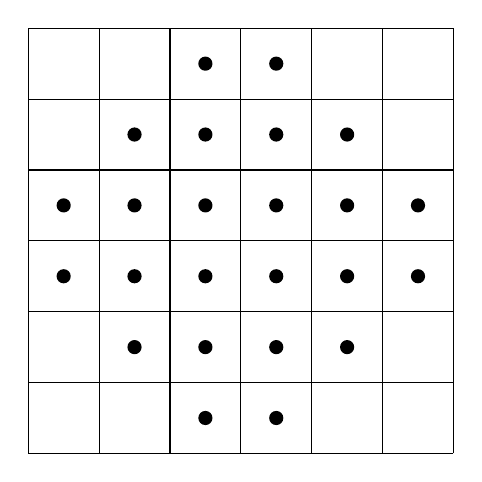
\begin{tikzpicture}[scale=0.9]
    \draw (0,0) grid (6,6);
    \foreach \x in {1,2,3,4} {
      \foreach \y in {1,2,3,4} {
        \fill (\x + 0.5, \y + 0.5) circle (0.1 cm);
      }
    }
    \foreach \n in {2,3} {
      \fill (0 + 0.5, \n + 0.5) circle (0.1 cm);
      \fill (5 + 0.5, \n + 0.5) circle (0.1 cm);
      \fill (\n + 0.5, 0 + 0.5) circle (0.1 cm);
      \fill (\n + 0.5, 5 + 0.5) circle (0.1 cm);
    }
  \end{tikzpicture} \hspace{1cm}
  \caption{
    Valid configurations for $4 \times 4$, $5 \times 5$, and $6 \times 6$ grids,
    proving that $a(4) = 16$, $a(5) \geq 21$, and $a(6) \geq 24$.}
\end{figure}

\begin{question}
  What is the greatest number of nonattacking pieces that can be placed on the board?
\end{question}

\begin{related}
  \item What if the board is $n \times m$?
  \item What if pieces must move like \textit{primitive} Pythagorean triples?
  \item What if each piece can move $k$ times?
  \item What is the asymptotic growth of $a$?
\end{related}
\end{document}
